% ====================================================================
%+
% SECTION:
%    section-name.tex  % eg lenstimedelays.tex
%
% CHAPTER:
%    chapter.tex  % eg cosmology.tex
%
% ELEVATOR PITCH:
%    Explain in a few sentences what the relevant discovery or
%    measurement is going to be discussed, and what will be important
%    about it. This is for the browsing reader to get a quick feel
%    for what this section is about.
%
% COMMENTS:
%
%
% BUGS:
%
%
% AUTHORS:
%    Phil Marshall (@drphilmarshall)  - put your name and GitHub username here!
%-
% ====================================================================

\section{Mapping the Milky Way Disk}
\def\secname{MW_Disk}\label{sec:\secname} % For example, replace "keyword" with "lenstimedelays"

\noindent{\it Will Clarkson, Peregrine McGehee, Jay Strader, Chris Britt}  % (Writing team)

% This individual section will need to describe the particular
% discoveries and measurements that are being targeted in this section's
% science case. It will be helpful to think of a ``science case" as a
% ``science project" that the authors {\it actually plan to do}. Then,
% the sections can follow the tried and tested format of an observing
% proposal: a brief description of the investigation, with references,
% followed by a technical feasibility piece. This latter part will need
% to be quantified using the MAF framework, via a set of metrics that
% need to be computed for any given observing strategy to quantify its
% impact on the described science case. Ideally, these metrics would be
% combined in a well-motivated figure of merit. The section can conclude
% with a discussion of any risks that have been identified, and how
% these could be mitigated.

%A short preamble goes here. What's the context for this science
%project? Where does it fit in the big picture?

Many populations of great importance to Astronomy exist predominantly
in or near the Galactic Plane, and yet are sufficiently
sparsely-distributed (and/or faint enough) that LSST is likely to be
the only facility in the forseeable future that will be able to
identify a statistically meaningful sample. Some (such as the novae
that allow detailed study of the route to Type Ia Supernovae) offer
unique laboratories to study processes of fundamental importance to
astrophysics at all scales. Others (like intra-disk microlensing
events) offer the {\it only} probe of important populations. An
important collateral benefit of studies in the plane with an LSST-like
facility, is improved mapping of the distribution and observational
effects of the ISM (particularly dust), which is of importance to all
IR/Optical/UV observational studies.

% --------------------------------------------------------------------

\subsection{Target measurements and discoveries}
\label{sec:\secname:MW_Disk_targets}

%Describe the discoveries and measurements you want to make.

%Now, describe their response to the observing strategy. Qualitatively,
%how will the science project be affected by the observing schedule and
%conditions? In broad terms, how would we expect the observing strategy
%to be optimized for this science?

We have identified five science cases within the general area of Milky
Way Disk studies, that will have a diversity of dependencies on
observing strategy (e.g. slow intrinsic variability vs fast intrinsic
variability vs no variability). When the figures of merit have been
computed for these science cases, the results will be summarized in a Table in Section~\ref{sec:\secname:MW_Disk_discussion}.

\begin{itemize}
  \item 1. Quantifying the large quiescent compact binary population via variability;
  \item 2. New insights into the behavior of Novae and the route to Type Ia Superovae;
  \item 3. The next Galactic Supernova;
  \item 4. Measuring population parameters of planets outside the Snow Line with Microlensing;
  \item 5. A three-dimensional Dust map and improvements in the reddening law
\end{itemize}

Motivation and qualitative description of response to observing strategy:

{\bf 1. Probing quiescent compact binaries via variability:} Of the
millions of stellar-mass black holes formed through the collapse of
massive stars over the lifetime of the Milky Way, only $\sim 20$ have
been dynamically confirmed through spectroscopic measurements
\citep[e.g.,][]{2015arXiv151008869C}.  Many questions central to modern
astrophysics can only be answered by enlarging this sample: which
stars produce neutron stars and which black holes; whether there is a
true gap in mass between neutron stars and black holes; whether
supernova explosions result in large black hole kicks. 

There is expected to be a large population of black hole binaries in quiescence
with low X-ray luminosities from $\sim 10^{30}$--$10^{33}$ erg/s.
Such systems can be identified as optical variables that show unique,
double-humped ellipsoidal variations of typical amplitude $\sim 0.2$
mag due to the tidal deformation of the secondary star, which can be a
giant or main sequence star. In some cases analysis of the light curve
alone can point to a high mass ratio between the components,
suggesting a black hole primary; in other cases the accretion disk
will make a large contribution to the optical light which results in
intrinsic, random, and fast variations in the light curve. The disk
contribution to optical light can change over time, and several years
of data is necessary to properly subtract the accretion disk
contribution in order to properly fit ellipsoidal veriations
\citep{2010ApJ...710.1127C}.
The brighter sources will be amenable to spectroscopy
with the current generation of 4-m to 10-m telescopes to dynamically
confirm new black holes; spectroscopy of all candidates should be
possible with the forthcoming generation of large telescopes. Thus,
LSST would trigger a rich variety of observational investigations of
the accretion/outflow process through studies of this large, dark
population.

While we have focused above on black hole binaries, we note that LSST would be
crucial for investigations of neutron star and white dwarf binaries. For
example, the total number of compact binaries is presently poorly
understood---Population models of neutron star X-ray binaries diverge by orders
of magnitude, largely due to uncertainties in the common envelope phase of
binary evolution
\citep[e.g.,][]{2003ApJ...597.1036P,2006MNRAS.369.1152K,2015A&A...579A..33V}.
This is poorly constrained but has a large impact on, for example,
LIGO event rates. A simple test case of common envelope evolution is available
in the number of dwarf novae (DNe) (accretion disk instability outbursts around
white dwarfs), a population that does not suffer from some of the complicating
factors that neutron star and black hole binaries do (e.g. supernova kicks).
Theoretical estimates routinely yield a significantly higher number of DNe than
are observed in the solar neighborhood. Understanding the true specific
frequency of these systems provides a key check on common envelope evolution.
LSST will detect dwarf novae, which last at least several days with typical
amplitudes of 4--6 mag, out to kpc scales. This will allow a test of not only
the number of cataclysmic variables, but also of the 3D distribution within the
Galaxy and dependence on metallicity gradients \citep{2015MNRAS.448.3455B}.

{\it Response to observing strategy:} Since most black hole candidates
have been identified near the plane in the inner Milky Way (68\%, 92\%
within $5^{\circ}, 10^{\circ}$~of the Plane), this science case {\it
    requires} that LSST observe the plane with sufficient cadence to
  detect the $\sim$hundreds of quiescent black-hole binaries by virtue
  of their variability. The natural choice for a survey for
  low-luminosity black hole binaries would be to extend the
  Wide-Fast-Deep survey throughout the Plane in the direction of the
  inner Milky Way. The orbital period of these systems is short (typically $<1$ day), so that a rolling cadence
  for at least parts of the Plane should be considered. For dwarf novae, the cadence of observations
  is critical in obtaining an accurate measure of the population of
  cataclysmic variables, as a long baseline is necessary to recover
  low duty cycle systems while widely-space observations
 would miss short outbursts.

%Describe the discoveries and measurements you want to make.

%Now, describe their response to the observing strategy. Qualitatively,
%how will the science project be affected by the observing schedule and
%conditions? In broad terms, how would we expect the observing strategy
%to be optimized for this science?

{\bf 2. Novae and the route to Type Ia Supernovae:} Only $\sim 15$
novae (explosions on the surfaces of white dwarfs) are discovered in
the Milky Way each year, while observations of external galaxies show
that the rate should be a factor of $\sim 3$ higher
\citep{2014ASPC..490...77S}.
Evidently, we are missing 50--75\% of novae due to their
location in crowded, extinguished regions, where they are not bright
enough to be discovered at the magnitude limits of existing transient
surveys. Fundamental facts about novae are unknown: how much mass is
ejected in typical explosions; whether white dwarfs undergoing novae
typically gain or lose mass; whether the binary companion is important
in shaping the observed properties of nova explosions. Novae can serve
as scaled-down models of supernova explosions that can be tested in
detail, e.g., in the interaction of the explosion with circumstellar
material \citep[e.g.,][]{2015arXiv151007662C}.  Further, since accreting white
dwarfs are prime candidates as progenitors of Type Ia supernovae, only
detailed study of novae can reveal whether particular systems are
increasing toward the Chandrasekhar mass as necessary in this
scenario.

{\it Response to observing strategy:} Most novae occur in the Galactic
Plane and Bulge, and therefore the inclusion of the Plane in a survey
of sufficient cadence to find these events promptly is of paramount
importance for this science. These events will trigger
multi-wavelength follow-up ranging from the radio to X-ray and
$\gamma$-rays; these data are necessary for accurate measurements of
the ejected mass.

{\bf 3. The First Galactic Supernova:} A supernova in the Milky Way
would be among the most important astronomical events of our lifetime,
with enormous impacts on stellar astrophysics, compact objects,
nucleosynthesis, and neutrino and gravitational wave astronomy. The
estimated rate of supernovae (both core-collapse and Type Ia) in the
Milky Way is about 1 per 20--25 years \citep{2013ApJ...778..164A}; hence there
is a 40--50\% chance that this would occur during the 10-year LSST
survey. If fortunate, such an event will be located relatively close
to the Sun and will be an easily observed (perhaps even naked-eye)
event. However, we must be cognizant of the likelihood that the
supernova could go off in the mid-Plane close to the Galactic Center
or on the other side of the Milky Way---both regions covered by
LSST. While any core-collapse event will produce a substantial
neutrino flux, alerting us to its existence, such observations will
not offer precise spatial localization. The models of Adams et
al.~(2013) indicate that LSST is the \emph{only} planned facility that
can offer an optical transient alert of nearly all Galactic
supernovae. 

{\it Response to observing strategy:} Even if the supernova is not too
faint, LSST will likely be the sole facility with synoptic
observations preceding the explosion, providing essential photometric
data leading up to the event---but only if LSST covers the Plane at a
frequent cadence. Just {\it how} frequent is open to exploration at
present, but the prospect of high-sensitivity observations of the
location of such a supernova {\it before} it takes place are clearly
of enormous scientific value. A secondary issue is the prospect that
an easily-observed Milky Way supernova might be too bright for LSST to
measure precisely with its planned exposure time, with a roughly 82\%
chance of a core-collapse supernova reaching one or two magnitudes
brighter than LSST's nominal saturation limit (with a 1/3 chance that
a ccSN would reach $m_V \sim 5$~(Adams et al. 2013). For a Type Ia in
the Milky Way, 
\citet{2013ApJ...778..164A} estimate $m_{V, max} \lesssim 13.5$~in 92\% of
cases.

{\bf 4. Population parameters of planets beyond the Snow Line with Microlensing:} Gould
(2013) shows that LSST could be an effective intra-disk microlensing
survey (in which disk stars are lensed by other objects in the disk,
such as exoplanets, brown dwarfs, or compact objects). The lower
stellar density compared to past bulge-focused microlensing surveys
would be offset by the larger area covered by LSST. The predicted rate
of high magnification microlensing events that are very sensitive to
planets would be $\sim 25$ per year. This survey would be able to
detect planets at moderate distances from their host stars, a regime
poorly probed by standard Doppler and transit techniques. The LSST
data alone would not be sufficient: the detection of a slow ($\sim$
days) timescale increase in brightness of a disk star would need to
trigger intensive photometric observations from small (1-m to 2-m
class) telescopes that would observe at high cadence for the 1--2
months of the microlensing event. This would represent an excellent
synergy between LSST and the wider observing community, and would
directly take advantage of the capabilities unique to LSST.

{\it Response to observing strategy:} To catch lensing events as they
start to brighten, with sufficient fidelity to trigger the intensive
follow-up required, the models of Gould (2013) suggest each field
should be observed once every few nights. With sparser coverage,
the survey would lose sensitivity to microlensing events in progress.

{\bf 5. Dust in the Milky Way disk:}
LSST studies of the interstellar medium, in particular the dust component,
are discussed in Section \ref{sec:MW_Dust}.

The Pan-STARRS1 survey (PS1) has
produced a three-dimensional dust map of the region of the sky covered
in their 3$\pi$ survey (which excludes a large part of the Galactic
Plane toward the south). Such maps are necessary to accurately measure
the intrinsic luminosities and colors of both Galactic and
extragalactic sources. The PS1 map (Schlafly et al.~2014) saturates at
extinctions $E(B-V) > 1.5$ as their tracer stars fall out of the
survey catalogs fainter than $g\sim 22$, meaning that this
high-fidelity map does not extend uniformly to within a few degrees of
the midplane. In addition, it only extends to a distance of about 4.5
kpc. Deep LSST data will allow this map to be extended to much higher
extinctions and larger distances. Owing to the high extinction and the
use of blue filters, this project is less affected by crowding than
other projects requiring photometry in the Plane. 

{\it Response to observing strategy:} When focusing on dust in the ISM (as
opposed to time-domain studies, e.g., dust around star-forming
regions or young stars), the main drivers of feasibility are
coverage of the few degrees around the Plane with sufficient photometric depth
and accuracy. This project is less affected by crowding than other
projects requiring photometry in the Plane owing to its use of blue
filters and the high extinction.  Nonetheless, quantiative estimates of
the expected photometric accuracy in coadded $u$ and $g$ images at low
Galactic latitude are desirable.


% --------------------------------------------------------------------

\subsection{Figures of Merit}
\label{sec:\secname:MW_Disk_metrics}

%Quantifying the response via MAF metrics: definition of the metrics,
%and any derived overall figure of merit.

Unpolished notes about likely (reasonably straightforward) figures of
merit (FoM) follow, along with (in some cases) possible directions for
future higher-level FoM. In many cases, dependencies on
Metrics are identified.  \new{WIC - Note to co-authors: these FoM
  were chosen to build off existing metrics in development. To take
  one example, Peter Y has developed some nice ipython Notebooks that
  illustrate representative Monte Carlo tests for periodicity
  detection including spatial variation - thus I think the Figures of Merit
  below should be straightforward to implement by modification of
  existing tools.}


{\bf FoM 1.1 - Fraction of quiescent
  black hole binaries detectable through ellipsoidal variability, as a function of location on sky and distance.}
Dependencies:
\begin{itemize}
  \item Monte Carlo in period, phase and shape parameters (ASCII input?) for variables as measured in a particular OpSim run. Likely run Monte Carlo for a representative number (ten?) of well-chosen orbital periods within the 0.1-5d range;
  \item (Since these are short-period objects): the ``PeriodicMetric'' of Lund et al. (2015);
  \item Will likely need reasonably high-spatial-resolution HEALPIX slices and a prescription for population density as a function of position on-sky (can be analytic).
\end{itemize}
Possible higher-order FoM: errors on the population size (mass
function??) derived from a survey under a given observing
strategy. Can imagine just adding up the ``recovered'' qLMXB
population and comparing it to that simulated. Some white noise componant of varying strengths could be
added to the light curves to simulate various contributions of the accretion disk to the continuum light. 
Note that the survey will necessarily be highly incomplete (inclination effects, etc.), it
is the likely {\it uncertainty} on the completeness-correction that
would be crucial in this case. 

{\bf FoM 1.2 - Fraction of dwarf novae detected in a given survey
  run as a function of location and distance.}
Dependencies:
\begin{itemize}
  \item Monte Carlo in distribution of maximum brightness and rise/decay timescale;
    \item "Triples" without filter constraints (given a prior detection in each filter)- what fraction are recovered?
    \item Histogram of duty cycle recovery efficiency versus duration of outburst and recurrence time.
    \item Histogram of recovery efficiency of maximum brightness of dwarf nova versus duration and recurrence time (if assume subsequent outbursts have similar profiles).
    \end{itemize}
Higher-level FoM: Uncertainty in LIGO event rates due to
uncertainties in common envelope evolution, which drives uncertainties in both LIGO event rates and DN population.

{\bf FoM 2.1 - Fraction of identified Novae as a function of location on-sky, distance, and time since initial rise.}
Dependencies:
\begin{itemize}
  \item Is the ``Triplets'' metric sufficient (i.e. is this ``just'' a case of supplying the metric the correct $\Delta t$~parameter values)?;
    \item What is the maximum interval since initial rise that would be acceptable? (Is this a function of waveband for followup?)
\end{itemize}
Possible higher-order FoM: error on inferred rate of Type Ia supernovae?

%{\bf FoM 3.1 - Maximum time-interval {\it before} triggering of a SN in the Milky Way that LSST would h%ave taken precursor data.}
%Dependencies:
%\begin{itemize}
%  \item This FoM would probably be very easy to calculate (just estimate the mean time between observat%ions). However the acceptable limits still need thought:
%  \item How many colors are sufficient? Any observations at all before the SN goes off, or would a comp%lete set in all filters be needed to characterize the candidate progenitor?
%    \item What level of variability sensitivity is really needed? Would just an extremely deep image of% the SN field before the event be sufficient?
%\end{itemize}
%{\bf FoM 3.2 - Maximum time-interval {\it after} the SN event for triggering followup.}
%Dependencies:
%\begin{itemize}
%  \item Similar to FoM 3.1. 
%    \item Is it important to know the discovery space for LSST? If a
%      supernova at $m_V~15$~goes off, other facilities are likely to
%      spot it...
%\end{itemize}


\new{\bf FoM 3.1 - Fraction of Galactic supernovae for which LSST would detect variability {\it before} the main Supernova event. Dependencies:}
\begin{itemize}
  \item \new{Assume the probability of a SN going off scales with the number of stars along the line of sight to some depth. The ``starcount'' metric in sims-maf-contrib (by Mike Lund and collaborators) calculates this value out to some fiducial distance. Additionally}; 
\item \new{This FoM requires an assessment of the ability of LSST to detect a particular lightcurve shape. Several options are possible at this time; we have selected ``metrics.TransientMetric'' from the baseline lsst-sims. Therefore also};
\item \new{a lightcurve shape for the pre-SN variability must be assumed.}
\end{itemize}

% WIC - removed this one since it's a bit low-level...
%
%{\bf FoM 3.2 - Maximum time-interval {\it after} the SN event for triggering followup.}
%Dependencies:
%\begin{itemize}
%  \item Similar to FoM 3.1. 
%    \item Is it important to know the discovery space for LSST? If a
%      supernova at $m_V~15$~goes off, other facilities are likely to
%      spot it...
%\end{itemize}



{\bf FoM 4.1 - Fraction of accurately-triggered Microlens candidates as a function of location, distance, lens mass.}
Dependencies:
\begin{itemize}
  \item Analytic (?) model for microlens lightcurve for representative sample of microlens parameters;
    \item transientASCIIMetric may well already do what we need! 
\end{itemize}

{\bf FoM 4.2 - errors in the (mass function, distance distribution) of intra-disk microlensed planets.}
Dependencies:
\begin{itemize}
  \item Event rate with sufficient-cadence observations to trigger followup as a function of (distance, lens mass);
\end{itemize}

{\bf FoM 5.1 - Errors in derived $E(B-V)$, $n_H$~as a function of
  location in the Plane.}
Dependencies:
\begin{itemize}
  \item SNR scaling with apparent magnitude
    \item For the M dwarf based technique, the relation between
      reddening-invariant index $[Q_{gri}]$~and intrinsic $g-i$~are
      expressed as polynomials, so expect non-linear relation with
      photometric error.  
      \item This uses a 5th-order polynomial to describe the
        $(Q_{gri}, g-i)$~stellar locus for M dwarfs $(g-i > 1.6)$.
        \item Care must be taken to correctly propagate errors through
          the various indices used - not trivial with so many choices
          of flux ratio used.
          \item Uncertainties in the parameterizations used for e.g. color-$M_V$~relationships.
            \item The above are all for every location probed on the map.
\end{itemize}

% --------------------------------------------------------------------

\subsection{OpSim Analysis}
\label{sec:\secname:MW_Disk_analysis}

\new{(To stimulate input from collaborators, we have implemented a mock-up of a simple figure of merit for the Galactic Supernova case. We choose FoM 3.1 - the fraction of galactic supernovae for which an SN2010mc-like pre-SN outburst could be discovered by LSST. The results of all FoM's for this Section are collected in Table \ref{tab_SummarMWDisk}.)}

\new{{\bf FoM 3.1: Fraction of Galactic supernovae for which LSST would detect variability {\it before} the main Supernova brightening:}}
\begin{itemize}
\item \new{{\it Definition:} 
\begin{equation}
  FoM_{preSN} \equiv \frac{ \sum^{sightlines}_{i} f_{var, i} N_{\ast, i} } {\sum^{sightlines}_{i} N_{\ast, i}}
\end{equation}
where $f_{var, i}$~is the fraction of transient events that LSST would detect for observing strategy including the $i$'th sightline, $N_{\ast,i}$~the number of stars present along the $i$'th sightline, and the FoM is normalized by the total number of stars returned by the density model over all sightlines. (For the two OpSim runs tested here, enigma-1189 and ops2-1092, the normalization factors differ by $\sim 0.1\%$.) Therefore $0.0 \le FoM_{preSN} \le 1.0$.}
\item \new{{\it Assumptions (observational):} Pre-SN variability similar to the
    pre-SN outburst of SN2010mc \citep{2013Natur.494...65O}. The pre-SN variability is
modeled as a sawtooth lightcurve (in apparent magnitude). We assume this
transient event will always reach brightness sufficient for LSST to observe, so
opt for a very bright peak apparent magnitude in all filters. We assume that
the probability of a supernova going off is proportional to the number of stars
along a particular line of sight.}
\item \new{{\it Parameters used:} The pre-SN outburst is simulated using the lsst-sims metrics.TransientMetric module. The lightcurve used has the following parameters: rise slope $-2.4$; time to peak; $20$~days; decline slope: $0.08$; total transient duration: 80 days. All filters are used in the detections, and 20 evenly-spaced phases are simulated for sensitivity to pathological cases (parameter nPhaseCheck=20). Peak apparent magnitudes used: $\{ 11,9,8,7,6,6\}$~in $\{u,g,r,i,z,y\}$. Then, $f_{var, i}$~is taken as the ``Sawtooth Alert'' quantity returned by metrics.TransientMetric. The starcounts metric (in sims-maf-contrib) is used to estimate the number of stars along a given line of sight, using fiducial distance limits ($10$pc $\le d \le 80$kpc).}
\item \new{{\it \bf Results:} $FoM_{preSN}$(enigma-1189) = 0.251, while $FoM_{preSN}$(ops2-1092)=0.852. See Figure \ref{f_opSim_GalacticSN} for a breakdown of this figure of merit across sightlines.}

\end{itemize}
\begin{figure}
\begin{center}
  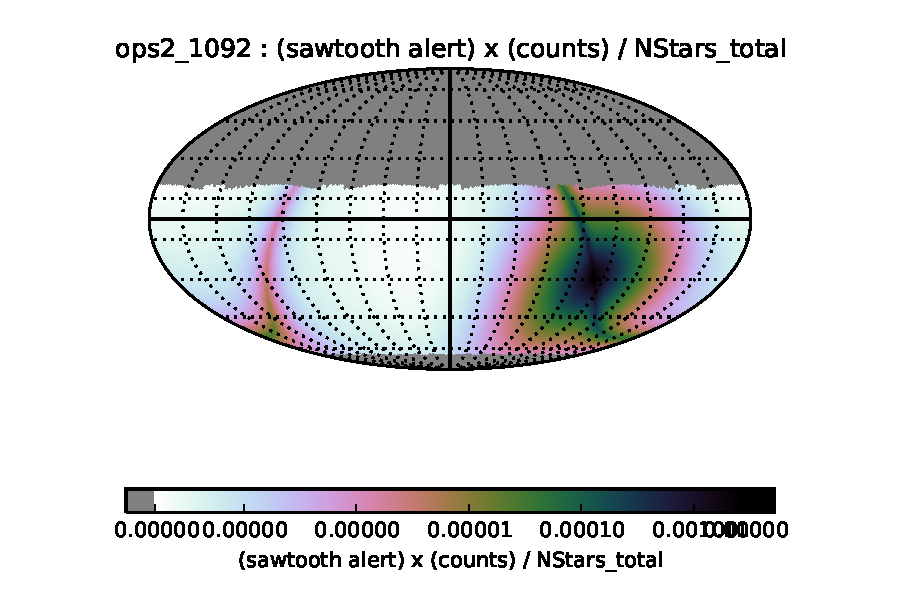
\includegraphics[width=7cm]{./figs/milkyway/galacticSN_SkyMap_1092.pdf}
  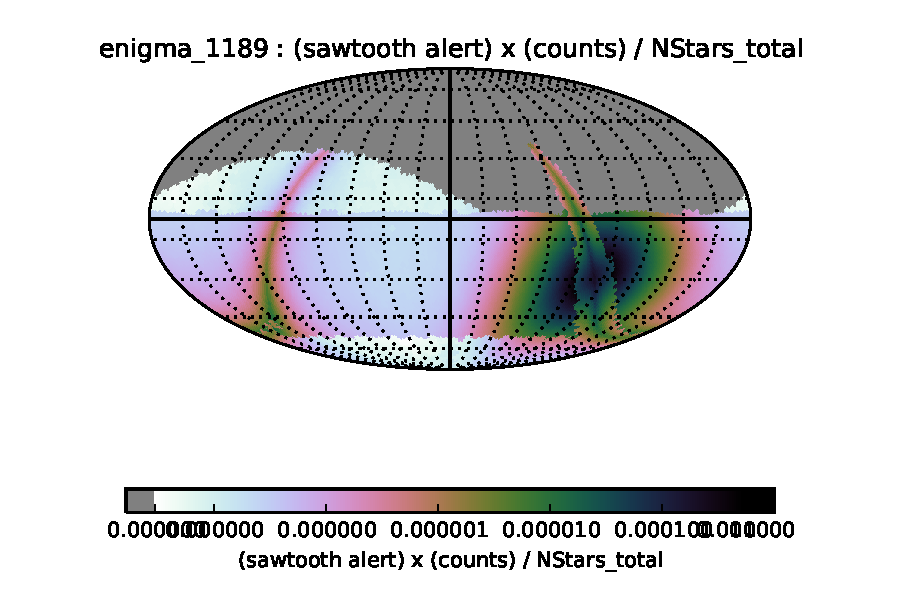
\includegraphics[width=7cm]{./figs/milkyway/galacticSN_SkyMap_1189.pdf}
%  \includegraphics[width=6cm]{./figs/milkyway/galacticSN_Histogram_1092.pdf}
%  \includegraphics[width=6cm]{./figs/milkyway/galacticSN_Histogram_1189.pdf} 
  \caption{\new{Figure of merit $FoM_{preSN}$~describing LSST's sensitivity to any pre-Supernova outburst, broken down by sightline, as sky-maps. $FoM_{preSN}$~is estimated for two OpSim runs (to-date); ops2-1092 (left) and enigma-1189 (right). The normalizing factors $N_{\ast, total}$ are $1.120\times 10^{12}$~for ops2-1092 and $1.121 \times 10^{12}$~for enigma-1189. The imprint of reduced sampling towards the inner plane can be clearly seen for enigma-1189.}}
\end{center}
\label{f_opSim_GalacticSN}
\end{figure}


%The current baseline cadence (${\tt enigma\_1189}$) partially excludes the Galactic Plane from the% deep-wide-fast survey and instead adopts a 
%nominal 30 visits per filter as part of a special proposal. We have proposed an OpSim run that inc%ludes the Galactic Plane in the 
%deep-wide-fast survey:

%\url{https://github.com/LSSTScienceCollaborations/ObservingStrategy/blob/master/opsim/Proposal_GP.md}

% The Figures of Merit listed above must now be implemented and applied to the OpSim databases.

%The metrics listed above should be carefully compared between our proposed run and the baseline cadence.


% --------------------------------------------------------------------

\subsection{Discussion: required work}
\label{sec:\secname:MW_Disk_discussion}

The Figures of Merit listed above must now be implemented within the
sims\_maf framework and applied to representative science
cases. \new{See Table \ref{tab_SummaryMWDisk} at the end of this subsection for initial
  efforts along these lines.}

We welcome input and volunteers for this effort. 

Qualitatively, however, we can note immediately that the current
baseline cadence (${\tt enigma\_1189}$) partially excludes the
Galactic Plane from the deep-wide-fast survey and instead adopts a
nominal 30 visits per filter as part of a special proposal - which
also tends to cluster the visits in the inner Plane within the first
few years of the survey. This already seriously compromises the time
baseline (see figure 4.3 of Section
\ref{sec:MW_Astrometry:MW_Astrometry_OpSim} for a demonstration applied to
proper motions).

We have proposed an OpSim run that includes the Galactic Plane in the
deep-wide-fast survey:

\url{https://github.com/LSSTScienceCollaborations/ObservingStrategy/blob/master/opsim/Proposal_GP.md}

\begin{table}
  \begin{tabular}{l|p{6cm}|c|c|c|c|p{5cm}}
    FoM & Brief description & {\rotatebox{90}{enigma-1189}} & {\rotatebox{90}{ops2-1092}} & {\rotatebox{90}{future run 1}} &  {\rotatebox{90}{future run 2}} & Notes \\
    \hline
    1.1 & \footnotesize{LMXB ellipsoidal variations}      & - & - & - & - & - \\
    1.2 & \footnotesize{Uncertainty in dwarf nova duty cycle}   & - & - & - & - &  \footnotesize{LSST as initial trigger} \\
    2.1 & \footnotesize{Fraction of Novae detected}       & - & - & - & - &  - \\
    3.1 & \footnotesize{Galactic Supernova pre-variability} & 0.25 & {\bf 0.85} & - & - & \footnotesize{Fraction of SN2010mc-like outbursts that LSST would detect; $FoM_{preSN} = f_{var} \times N_{\ast}$} \\
    4.1 & \footnotesize{Fraction of triggered microlens candidates} & - & - & - & - & - \\
    4.2 & \footnotesize{Uncertainty in disk-disk microlens distribution parameters due to missed events} & - & - & - & - & \footnotesize{LSST as initial microlens trigger} \\
    5.1a & \footnotesize{Median (over sight-lines) of the uncertainty in $E(B-V)$} & - & - & - & - & \footnotesize{(Most useful FoM probably a spatial map of the uncertainty.)} \\
    5.1b & \footnotesize{Variance (over sight-lines) of the uncertainty in $E(B-V)$} & - & - & - & - & - \\
  \end{tabular}
\caption{Summary of figures-of-merit for the Galactic Disk science cases. The best value of each FoM is indicated in bold. See Section \ref{sec:MW_Disk}.}
\label{tab_SummaryMWDisk}
\end{table}


%Discussion: what risks have been identified? What suggestions could be
%made to improve this science project's figure of merit, and mitigate
%the identified risks?



% ====================================================================

\navigationbar
